% =============================================================================================
% SUPPLEMENTARY MATERIAL.  Compiles standalone: pdflatex supplementary && bibtex supplementary
% && pdflatex supplementary twice. Shares references.bib with the manuscript.
%
% Numbers come from data/exports/kappa_v2/paper_numbers.json and the CSVs in data/Target_Materials
% (CONDITIONAL_PREDICTIONS.csv, PAPER_PREDICTIONS.csv, STRUCTURE_ONLY_29_VERIFIED.csv,
% STRUCTURE_ONLY_12_PREDICTIONS.csv, SURROGATE_11_PREDICTIONS.csv, CALIBRATED_NEW_PREDICTIONS.csv).
% S7 reads model_comparison (R2, RMSE, MAE on log10 kappa; median error per compound) from the
% registry; Figs. fig13_parity_models and fig14_feature_corr are generated by paper/fig13_*.py and
% paper/fig14_*.py. One descriptive file outside the registry is named where it occurs:
% extraction_agreement.json (S9).
%
% Keys added in the 2026-10-05 refinement:
%   S1 coverage 51.3 / 92.3        conformal bands empirical_coverage_pct (0.50, 0.90)
%   S1 form choice                 family_form_nested (SHAPE vs SHAPE_NOCAP, nested_choice 21.7)
%   S1 VEC rule                    make_paper_predictions.ve(): group (1-12), group - 10 (13-18);
%                                  pymatgen gives every lanthanide group 3
%   S3 YNiBi in the blind test     blind_by_family Ni-Bi n = 1; headline_without_YNiBi (n 38,
%                                  33.1, seed range 24.6-35.5, 86.8, p 0.0052 / 0.006)
%   S6 188 of 189                  provenance_sources.measurement_sources_in_reference_list
%   S7 0.1 pp                      model_comparison median error 26.0 (LightGBM) vs 26.1 (CatBoost)
%   S8 2.18, 189 points            cap_test.max_uncapped_factor; offset.n_points
%   S11 24 counted after the       structure_only.counts.by_category sums to listed_no_published_kappa
%     exclusion
%   S11 SmOF                       ml element holdout (element_holdout_X: SmNiBi, SmOF, SmSnAu)
%
% The main text cites S3 by number and the Extended Methods (S12) by name. S12 (Extended Methods)
% and S13 (flagged compounds: tab:refusals, fig:landscape) were moved here from the main text in
% the 2026-10-05 condensing pass and are appended last so that S1-S11 keep their numbers.
% =============================================================================================

\documentclass[preprint, 12pt]{elsarticle}

\usepackage[T1]{fontenc}
\usepackage[utf8]{inputenc}
\usepackage{amsmath, amssymb}
\usepackage{graphicx}
\usepackage{booktabs}
\usepackage[separate-uncertainty=true, detect-weight=true]{siunitx}
\usepackage[version=4]{mhchem}
\usepackage{microtype}
% Flush each section's floats before the next section starts, so that every table and figure sits
% with the section that introduces it (S13-S16 are short and would otherwise share one page while
% their floats queue behind them).
\usepackage[section]{placeins}
\usepackage[hidelinks]{hyperref}

\sisetup{group-separator = {,}, group-minimum-digits = 4}

% Number everything S1, S2, ... so nothing collides with the main text.
\renewcommand{\thesection}{S\arabic{section}}
\renewcommand{\thetable}{S\arabic{table}}
\renewcommand{\thefigure}{S\arabic{figure}}

\journal{Computational Materials Science}

\begin{document}

\begin{frontmatter}
\title{Supplementary material for\\
       \emph{Predicting the experimental lattice thermal conductivity of half-Heusler compounds
       by machine learning and transfer-function calibration}}
\end{frontmatter}

\section{Conditional estimates for the \ce{Ni}--\ce{Bi} family}
\label{sec:conditional}

Table~\ref{tab:conditional} lists ten compounds that cannot be issued, because their bonding family,
\ce{Ni}--\ce{Bi}, has no usable measured member (Section~\ref{sec:nibi}). A bonding family is the set
of half Heuslers XYZ that share their Y (late transition metal) and Z (main-group) elements; its
label names those two elements, in no meaningful order. Nine of the ten pass every structural and
chemical screen of the main text; the tenth, \ce{SmNiBi}, is flagged (below). They are not
predictions. Each row is the value the method would issue once the family can be calibrated. We
record it before the measurement that would license it, so that it can later be checked rather than
fitted.

All ten start from a published transport calculation at \SI{300}{\kelvin}, so the regression model
does not enter them; only the calibration step carries an error. With no family constant available,
they are quoted at the shared constant ($c=\num{0.42}$, $p=\num{0.70}$) as a stated proxy. The error
that goes with this choice is the shared constant's error on bonding families with no measured
member, each family left out of the fit in turn: a median of \SI{33.0}{\percent}, with
\SI{79.4}{\percent} of compounds within a factor of two, over \num{34} compounds. Two sound
\ce{Ni}--\ce{Bi} measurements, meaning measurements free of the bipolar contribution that rules out
the existing \ce{YNiBi} curve (Section~\ref{sec:nibi}), would replace the shared constant with a
family constant. Where a family constant can be tested, fitted without the compound it predicts, it
lowers the median error from \SI{32.3}{\percent} to \SI{21.7}{\percent} on the \num{31} compounds of
the main-text family test. Choosing the form of the correction (capped or uncapped;
Section~\ref{sec:cap}) inside each fold gives the same \SI{21.7}{\percent}. Compound by compound,
the gain is not significant: the family constant is closer for \num{16} compounds, further for
\num{11} and tied for \num{4} (two-sided sign test, $p=\num{0.44}$). Later sections refer to these
figures here rather than repeat them.

One row is flagged. The valence-electron count (VEC) used by the screens sums, over the three
elements, the group number for groups 1--12 and the group number minus 10 for groups 13--18, and
counts every lanthanide as 3. \ce{Sm} can be di- or trivalent, so the count of 18 for \ce{SmNiBi}
is not secure. Its admission to the domain therefore rests on an assumption the other nine do not
need. It is flagged on the same grounds as \ce{SmBiPd} (Section~\ref{sec:structureonly}). A
\ce{Ni}--\ce{Bi} family constant would release the other nine, but not this row.

\begin{table}[htb]
  \centering
  \caption{Conditional estimates for the ten \ce{Ni}--\ce{Bi} compounds at \SI{300}{\kelvin}.
  $\kappa_L^{\mathrm{BTE}}$ is the published transport calculation; the estimate is
  $\kappa_L^{\mathrm{BTE}}$ multiplied by the shared transfer function, whose value at
  \SI{300}{\kelvin} is \num{0.42}. Intervals are the main-text conformal bands at the quoted
  temperature, median over five model seeds: a factor of \num{1.62} either way for the
  \SI{50}{\percent} band, and \num{2.85} for the \SI{90}{\percent} band. On the \num{39} in-domain
  compounds, \num{20} (\SI{51.3}{\percent}) fell inside the \SI{50}{\percent} band and \num{36}
  (\SI{92.3}{\percent}) inside the \SI{90}{\percent} band, each compound under its own calibration.
  This coverage is not validated for a family with no measured member; there, the shared constant's
  held-out error is a median \SI{33.0}{\percent}, with \SI{79.4}{\percent} of compounds within a
  factor of two. $n_{\mathrm{src}}$ is the number of independent calculations, counting a preprint
  and the journal article it became as one source. \emph{Spread} is the maximum ratio between them;
  a spread above \num{2} would remove the row (Section~\ref{sec:spread}).}
  \label{tab:conditional}
  \small
  \setlength{\tabcolsep}{4pt}
  \begin{tabular}{lcccccc}
    \toprule
    Compound & $\kappa_L^{\mathrm{BTE}}$ & Estimate & \SI{50}{\percent} & \SI{90}{\percent} &
      $n_{\mathrm{src}}$ & spread \\
    & \multicolumn{4}{c}{(\si{\watt\per\meter\per\kelvin})} & & \\
    \midrule
    \ce{NdNiBi} &  5.25 & 2.21 & 1.36--3.57 & 0.77--6.28  & 1 & --- \\
    \ce{PrNiBi} &  5.28 & 2.22 & 1.37--3.59 & 0.78--6.32  & 2 & 1.36 \\
    \ce{GdNiBi} &  8.12 & 3.41 & 2.11--5.52 & 1.20--9.72  & 1 & --- \\
    \ce{TmNiBi} &  8.22 & 3.45 & 2.13--5.59 & 1.21--9.83  & 2 & 1.32 \\
    \ce{SmNiBi}$^{\dagger}$ &  8.49 & 3.57 & 2.20--5.78 & 1.25--10.17 & 1 & --- \\
    \ce{LuNiBi} &  9.83 & 4.13 & 2.55--6.69 & 1.45--11.77 & 1 & --- \\
    \ce{TbNiBi} &  9.88 & 4.15 & 2.56--6.72 & 1.46--11.83 & 2 & 1.31 \\
    \ce{ScNiBi} & 10.91 & 4.58 & 2.83--7.43 & 1.61--13.06 & 2 & 1.41 \\
    \ce{ErNiBi} & 10.93 & 4.59 & 2.83--7.44 & 1.61--13.09 & 2 & 1.26 \\
    \ce{DyNiBi} & 11.78 & 4.95 & 3.05--8.01 & 1.74--14.10 & 1 & --- \\
    \bottomrule
  \end{tabular}

  % Notes sit outside the tabular: table cells do not line-break, and a note inside forces the
  % tabular past the text block.
  \vspace{2pt}
  \begin{minipage}{\linewidth}\footnotesize
    $^{\dagger}$ Flagged: \ce{Sm} may be di- or trivalent, so $\mathrm{VEC}=18$ is assumed here, not
    counted.\par
    Two sound \ce{Ni}--\ce{Bi} measurements release the nine unflagged rows together: either a
    re-measurement of \ce{YNiBi} below its bipolar onset plus one further \ce{Ni}--\ce{Bi} compound,
    or two new compounds.
  \end{minipage}
\end{table}

\section{The measurements that would release or strengthen predictions}
\label{sec:fourteen}

Four kinds of measurement would change what the method can say, and each buys something different.

Two sound \ce{Ni}--\ce{Bi} measurements would release nine of the ten estimates of
Table~\ref{tab:conditional} at once, by giving the family its own constant. The tenth, \ce{SmNiBi},
stays flagged. No other measurement releases as many.

One further measured compound in \ce{Co}--\ce{Bi} or in \ce{Ni}--\ce{Pb} would add no predictions,
but would change the standing of four issued ones. Each of these families is anchored, that is,
calibrated on a single measured member: \ce{ZrCoBi} and \ce{ZrNiPb} respectively, which its own
family constant fits to \SI{6.3}{\percent} and \SI{5.6}{\percent} in sample. \ce{HfCoBi} and
\ce{TiCoBi} (\ce{Co}--\ce{Bi}), and \ce{HfNiPb} and \ce{TiNiPb} (\ce{Ni}--\ce{Pb}), are issued
through those constants, and the main text says so. A second member would let each constant be
tested held out, as it is for the nine families with more than one member. Each anchor also rests
on a single laboratory. The \ce{ZrCoBi} reference is a specimen of \SI{98.1}{\percent} density. The
other laboratory that measured \ce{ZrCoBi} used a ball-milled specimen, and reads lower by a factor
of \num{1.7} at \SI{300}{\kelvin}. The two \ce{Co}--\ce{Bi} predictions therefore inherit the
reference laboratory's basis. For \ce{Ni}--\ce{Pb}, a bulk specimen is the useful measurement:
\ce{ZrNiPb} was measured on a ball-milled sample, so the two \ce{Ni}--\ce{Pb} predictions describe a
milled specimen.

One further measured compound in \ce{Sb}--\ce{Ir} would decide two compounds that are now declined.
The family's single member, \ce{ZrSbIr}, is fitted to only \SI{36.6}{\percent} even in sample, so
\ce{TiSbIr} and \ce{HfSbIr} are flagged rather than issued. A second member would show whether the
family can be calibrated at all.

One further measured compound in \ce{Bi}--\ce{Pd} would bear on the largest group of flagged
values. The family's three members, \ce{ErBiPd}, \ce{GdBiPd} and \ce{LaBiPd}, come from two papers.
Held out, they are predicted to \SI{25.3}{\percent}, just outside the \SI{25}{\percent} threshold
on a family's held-out median error, and their individual constants span a factor of \num{1.41}.
The family's nine candidates are therefore flagged in the main text, and most of them also lie
above the family's measured range. A fourth member, ideally from another laboratory, would show
whether the family constant clears the threshold.

\section{The \ce{Ni}--\ce{Bi} family: status of its one measured member}
\label{sec:nibi}

\ce{Ni}--\ce{Bi} is blocked by an unusable reference, not a missing one. The distinction matters
because harvesting more literature does not fix it.

The family's only measured member is \ce{YNiBi}, whose reported $\kappa_L$ \emph{rises} with
temperature across the whole curve. Lattice conduction cannot show this temperature dependence. The
source itself gives the reason: its authors report a significant bipolar contribution to the thermal
conductivity of \ce{YNiBi}~\cite{li2015synthesis}. A single-parabolic-band Lorenz number has no
bipolar term. Above the bipolar onset, the electronic part is therefore under-subtracted, and the
remainder, booked as lattice conductivity, climbs with temperature. The defect lies in the
electronic--lattice separation, not in the specimen or in our transcription. It rules the curve out
as a family reference: no \ce{Ni}--\ce{Bi} constant is fitted to it, and we do not count it as
validation of one, even though the calibrated calculation happens to match it
(\SI{13.0}{\percent} error, ratio \num{0.87}, at \SI{281}{\kelvin}, the measured point nearest
\SI{300}{\kelvin}). \ce{YNiBi} does remain one of the \num{39} compounds of the main-text blind
test, because a compound whose every curve fails the shape test keeps its measurement there, ranked
last, so that the scored population does not depend on that test. Without it, the blind test gives
a median error of \SI{33.1}{\percent} (seed range \SIrange{24.6}{35.5}{\percent}) with
\SI{86.8}{\percent} of \num{38} compounds within a factor of two, and $p=\num{0.005}$ and
\num{0.006} against the constant and power-law nulls.

A wider literature search does not close the gap. \ce{YNiBi} is the only rare-earth \ce{Ni}--\ce{Bi}
half Heusler with a measured $\kappa_L$ in the sources we harvested, and we found no work citing it
that reports a second measurement. \ce{LuNiBi}, the best-studied candidate, has been probed by
inelastic X-ray scattering together with first-principles calculations~\cite{li2024multiphono}, but
no source we harvested has a measured $\kappa_L$ for it. The one \ce{Ni}--\ce{Bi} compound with an
independent $\kappa_L$ measurement is \ce{ZrNiBi}, and it is excluded on grounds its own authors
establish. Stoichiometric \ce{ZrNiBi} has $\mathrm{VEC}=19$, lies above the convex hull, and can be
made phase-pure only as the \ce{Zr}-deficient \ce{Zr0.88NiBi}~\cite{ren2023vacancymed,liu2025stabilizat}.
It therefore fails both the valence-count screen and the restriction to stoichiometric compounds.
Because the synthesis literature motivates its exclusion independently, the exclusion checks the
screen rather than coinciding with it.

\ce{Ni}--\ce{Bi} therefore has zero usable members and needs two (Table~\ref{tab:conditional}).

\section{Disagreement between independent calculations}
\label{sec:spread}

Where more than one group has calculated a compound, the published values need not agree. We count a
preprint and the journal article it became as one source. Across the \num{82} half Heuslers with two
or more independent transport calculations at \SI{300}{\kelvin}, the median disagreement is a factor
of \num{1.37}. One compound in ten exceeds \num{2.43}, and the tail reaches \num{18.35}
(\ce{TmNiSb}).

This bears on the predictions in two ways. First, we do not use any temperature at which a
compound's independent calculations disagree by more than a factor of two; this applies to
candidates exactly as to measured compounds. The compound is then quoted from its uncontested
calculations, those that no independent calculation contradicts by more than that factor.
\ce{TiNiPb} is the example: its two calculations at \SI{300}{\kelvin} differ by a factor of
\num{5.6}, so it is quoted at \SI{500}{\kelvin}, where its one calculation is uncontested.

Second, a spread below that threshold is not carried into any interval. \ce{ErSbPt} and
\ce{HoSbPt}, both issued with the main text's marginal-extrapolation label (a value outside its
family's measured span by less than the median factor between laboratories), each rest on three
independent calculations, which differ by factors of \num{1.68} and \num{1.72} respectively. The
conformal interval describes the error of the transfer function only; it does not include the spread
among its inputs. Where independent calculations disagree, the stated \SI{90}{\percent} band should
therefore be read as a lower bound on the true uncertainty. The same holds for the conditional rows
of Table~\ref{tab:conditional} that carry a spread.

\section{Which measurement is the most informative}
\label{sec:informative}

\ce{Ni}--\ce{Bi} is the most productive measurement the corpus points to
(Section~\ref{sec:fourteen}). For the estimates from crystal structure alone, the informative first
measurements lie in the families that hold them, none of which has been measured. \ce{Te}--\ce{Os}
holds two (\ce{HfTeOs}, main text; \ce{ZrTeOs}, Section~\ref{sec:structureonly}), \ce{Pb}--\ce{Au}
one (\ce{TmPbAu}, main text) and \ce{Bi}--\ce{Pt} one (\ce{ScBiPt}). All of them carry the shared
constant, with the error that travels with it on a family with no measured member
(Section~\ref{sec:conditional}). A first measurement would give the family its own constant, with
the gain, and the caveat on its significance, given there.

A first \ce{Bi}--\ce{Pt} measurement would also say something about the transfer function. The
constants of the two palladium families are far apart: \num{0.24} for \ce{Sb}--\ce{Pd} and
\num{0.95} for \ce{Bi}--\ce{Pd}, the largest of the twelve family constants. Measured
\ce{Bi}--\ce{Pd} compounds therefore sit close to their calculations. It is open whether this is a
property of bismuth on a noble-metal site, or of the \ce{Bi}--\ce{Pd} pairing alone. A single
\ce{Bi}--\ce{Pt} measurement would show whether the shared constant is a sound proxy for
\ce{Bi}--\ce{Pt}.

\section{Provenance of every measurement and calculation}
\label{sec:provenance}

The corpus is assembled from other people's work, and the claim that every value in it is traceable
can be checked only if those works are named. Because there are so many, they are cited here rather
than in the main text. They are \num{188} of the \num{189} publications behind the measurements (the
remaining one is explained below), the \num{29} behind the full transport calculations, and those
behind the semi-empirical estimates used as a baseline. A publication that serves in more than one
role is listed once. Calculations on machine-learned force fields form a separate method tier, used
in neither training nor calibration.

Every entry appears in full in the reference list below. Every row of the released corpus carries
the identifier of the work it came from, so a reader can trace any number in the dataset to the
paper that reported it. One further measurement source is missing from the list for a mechanical
reason: its digital object identifier (DOI) is registered with neither Crossref nor DataCite, so it
cannot be resolved into a reference entry. It is named in the released corpus.

% ============================================================================================
% PROVENANCE.  Input by supplementary.tex (Section S6).
%
% The main text claims that every value in the corpus carries an explicit provenance. A reference
% list containing only the works discussed in the text does not demonstrate that claim; it
% leaves the publications the measurements actually come from invisible. These \nocite blocks
% put them into the reference list, which is what makes the claim checkable by a reader.
%
% Keys are the distinct source DOIs of the deduplicated corpus by method tier, mapped to
% references.bib exactly as make_paper_numbers.py does for provenance_sources:
%   tier 0 (measurements): 188 keys = provenance_sources.measurement_sources_in_reference_list
%     (189 DOIs; 10.36410/jcpr.2020.21.3.319 has no bib entry);
%   tier 1 (full transport calculations): 29 keys = provenance_sources.calculation_source_dois.
%     Three of them (yue2023strong, yang2024hh, lyu2026pressurein) were listed by the registry as
%     analysed-but-never-cited; they are added here, so calculation_sources_in_reference_list
%     reads 29 once the registry is regenerated. Rows on machine-learned force fields are tier 2
%     and are not listed (they are not used in training or calibration).
%   semi-empirical baseline (in_domain_table.published_semi_empirical, n = 22): the four sources
%     whose estimates are matched to the in-domain compounds by compute_baselines_ablation.py.
% han2023strong sits in both the tier-0 and tier-1 blocks; choudhary2021first in the tier-1 and
% baseline blocks. NOTE: paper/bibliography_report.json keys_by_method_tier predates the current
% tiers (it lists 198 tier-0 and 20 tier-1 keys); these blocks follow the current corpus.
% ============================================================================================

% --- experimental measurements analysed in this work (method tier 0) ---
\nocite{akram2015enhanced,anon2011thermoelec,aversano2020role,bag2020thermoelec,balke2011an}
\nocite{barczak2018impact,barth2009thermoelec,barth2010investigat,barth2010itinerant,berry2017enhancing}
\nocite{berry2017improving,bhardwaj2014improving,bhattacharya2002grain,birkel2012rapid,birkel2013improving}
\nocite{birkel2013influence,buffon2016enhancemen,chauhan2018vanadiumdo,chauhan2019compositio,chauhan2019enhanced}
\nocite{chauhan2019spinodal,chen2018improved,chen2021fast,ciesielski2020thermoelec,delimecodrin2017carrier}
\nocite{douglas2012enhanced,douglas2014phase,dow2018effect,elkhouly2020transport,ferluccio2018impact}
\nocite{ferluccio2021thermal,fu2012enhanced,gao2020significan,gelbstein2011thermoelec,germond2010thermoelec}
\nocite{gong2019continuous,gong2019effects,graf2010phasesepar,grth2016thermoelec,grytsiv2019thermoelec}
\nocite{han2023strong,hari2020thermoelec,hazama2012thermoelec,he2016enhanced,he2020unveiling}
\nocite{he2026defectcalc,hinterleitner2020stoichiome,hooshmandzaferani2020experiment,huang2004the,huang2015a}
\nocite{huang2017the,huang2018the,huang2019improving,huang2020electron,huang2021point}
\nocite{huang2022discovery,johari2020band,kanemitsu2006transport,katayama2003the,katsuyama2004effect}
\nocite{katsuyama2007thermoelec,katsuyama2010effect,kawaharada2003high,kawaharada2004high,kawaharada2004higha}
\nocite{kawaharada2004highb,kawano2007effect,kim2004enhancemen,kim2007high,kimura2006thermoelec}
\nocite{kimura2006thermoeleca,kimura2008thermoelec,kimura2010vacancy,kirkham2012mmlmath,kurosaki2009effect}
\nocite{laila2020preparatio,landmann2019fabricatio,lei2016microwave,li2010effect,li2013high}
\nocite{li2015synthesis,li2019ntype,li2020titanium,li2024enhancemen,li2025impact}
\nocite{liu2012fabricatio,liu2012lowtempera,lkhagvasuren2017improved,lu2009thermoelec,lue2002thermoelec}
\nocite{lue2004offstoichi,lue2004thermal,lue2007thermoelec,lue2008effects,mao2017thermoelec}
\nocite{mastronardi1999antimonide,mato2025starrydata,mena2016miscibilit,miao2026exceptiona,mikami2012thermoelec}
\nocite{mikami2013effect,mikami2015thermoelec,misra2014enhanced,misra2015enhanced,mohamed2020tuning}
\nocite{mondal2018ferromagne,mondal2023thermoelec,morozkin2005thermoelec,mukhopadhyay2018multifunct,muta2005thermoelec}
\nocite{muta2009hightemper,nagai2011preparatio,oestreich2003thermoelec,ojha2024low,ono2006thermoelec}
\nocite{ono2006thermoeleca,ouardi2011transport,ouardi2012electronic,pallecchi2018thermoelec,popescu2024effects}
\nocite{qiu2009enhanced,qiu2010effect,rahul2026linking,ramachandran2018thermoelec,rogl2020halfheusle}
\nocite{sato2021effect,schmitt2015resolving,schrade2017the,schwall2012thermomagn,schwall2018on}
\nocite{sekimoto2005annealing,sekimoto2005thermoelec,sekimoto2005thermoeleca,sekimoto2006lnpdsb,sekimoto2006thermoelec}
\nocite{sekimoto2006thermoeleca,sekimoto2006thermoelecb,sekimoto2006thermoelecc,sekimoto2007highthermo,sekimoto2007thermoelec}
\nocite{serranosnchez2020thermoelec,shen2001effects,silpawilawan2017fenbsb,skovsen2010multitempe,sportouch1998observed}
\nocite{synoradzki2019thermal,taranova2019influence,tavassoli2017on,thiem2025thermoelec,toberer2009thermoelec}
\nocite{tseng2017semimetall,uher1999transport,vishwakarma2020compositio,voronin2017preparatio,wang2025enhanced}
\nocite{wei2015thermoelec,wolaska2019enhanced,wu2007thermoelec,wu2009effects,xia2000thermoelec}
\nocite{xia2018enhanced,xie2012increased,xie2012interrelat,xie2014the,xu2020anomalous}
\nocite{yadav2021optical,yadav2022unravellin,yamamoto2017the,yan2020realizing,yang2020enhanced}
\nocite{yang2020identifica,yoshioka2015solid,yousuf2018ternary,yu2010reduced,yu2012high}
\nocite{yuan2017effects,zhang2016synthesis,zhao2014synthesis,zhao2018synthesis,zhao2018synthesisa}
\nocite{zhao2021thermoelec,zheng2023symmetrygu,zheng2025boosting,zhou2005effects,zhou2007moderatete}
\nocite{zhu2018discovery,zhu2019discovery,zou2017band}

% --- full transport calculations analysed in this work (method tier 1) ---
\nocite{ali2026comprehens,carrete2014finding,chen2021computatio,ding2015examining,ding2016thermoelec}
\nocite{eliassen2017lattice,han2020high,han2023strong,he2019designing,hermet2016lattice}
\nocite{jaishi2021electronic,keshri2020intrinsica,li2025highthroug,lyu2026pressurein,miyazaki2021machine}
\nocite{ohnishi2026database,raghuvanshi2021selfdoping,rodriguez2023millionsca,shastri2020firstprinc,trans2022lattice}
\nocite{wang2022intrinsic,xue2016laptsb,yang2024hh,yue2023strong}
% preprints with no published version on record (the arXiv DOI is the version cited)
\nocite{guo2016thermoelec,kaur2017pursuit,choudhary2021first,vishwakarma2023ab,saini2026pressuredr}

% --- semi-empirical estimates used as a baseline (method tier 3) ---
\nocite{choudhary2021first,hong2016fullscale,nan2025datadriven,pak2025mapping}


\section{Regressor comparison}
\label{sec:smodel}

The machine-learning model supplies $\kappa_L^{\mathrm{BTE}}$ from crystal structure where no
published calculation exists; this section reports its selection in more detail than the main text
does. We trained four regressors (CatBoost, LightGBM, a Gaussian process and kernel ridge
regression) on identical rows and descriptors. We used five-fold cross-validation grouped by element
system, so that whole chemistries are held out, and every regressor saw the same folds. These
element-system folds are a different holdout from the X-site chemistry clusters of the main-text
blind test. The rows are the production training build (\num{681} rows on \num{463} compounds). They
comprise the tier-1 labels (full first-principles transport calculations) plus, at reduced weight,
the semi-empirical estimates for full Heuslers that have no calculation. Pool, weighting, descriptor
set and grouping match the production model, so the comparison describes the model specification the
paper uses.

RMSE, MAE and $R^2$ are computed per row, on $\log_{10}\kappa_L$, from the out-of-fold predictions.
The median error is computed per compound: the median, over compounds, of each compound's median row
error. CatBoost leads on all three per-row metrics: $R^2$ \num{0.701} against
\numrange{0.516}{0.695}, RMSE \num{0.270} against \numrange{0.273}{0.343}, and MAE \num{0.182}
against \numrange{0.186}{0.236}. LightGBM leads narrowly on median error per compound
(\SI{26.0}{\percent}, against \SI{26.1}{\percent} for CatBoost, \SI{26.4}{\percent} for the Gaussian
process and \SI{32.3}{\percent} for kernel ridge). We retain CatBoost, which leads on the per-row
metrics; LightGBM's lead on the per-compound median is \num{0.1} percentage points, too small to
separate the two. Three of the four are close on every metric, and the comparison concerns fit to
\emph{calculated} labels, not to measurements.

Figure~\ref{fig:parity_models} plots each regressor's out-of-fold predictions against its labels.
CatBoost, LightGBM and the Gaussian process scatter alike about the diagonal. Kernel ridge
compresses the range: it predicts the lowest labels too high and the highest too low, which explains
its larger RMSE. All four predict the few highest labels too low.

Figure~\ref{fig:feature_corr} gives the Pearson correlation between the descriptors that vary across
the pool. The five disorder descriptors are omitted: they are zero for every row, because every
training compound is stoichiometric. Several pairs are nearly redundant: mean atomic mass and formula
mass; mean radius and sum of radii; X--Z electronegativity difference and electronegativity spread;
volume per atom and bond-length scale; shortest and mean bond length; atoms per cell and the
full-Heusler flag; and the three encodings of temperature. Such redundancy does not harm a tree
ensemble's predictions, but it splits the attribution between the members of each pair. The main
text (subsection ``What the model has learned'') discusses the \textsc{shap} (SHapley Additive
exPlanations) attribution of the retained model and draws its eight largest terms, and applies this
caveat there. Figure~\ref{fig:shap} gives the full attribution for the twelve descriptors with the
largest mean absolute contribution, row by row.

\begin{figure*}[tp]
  \centering
  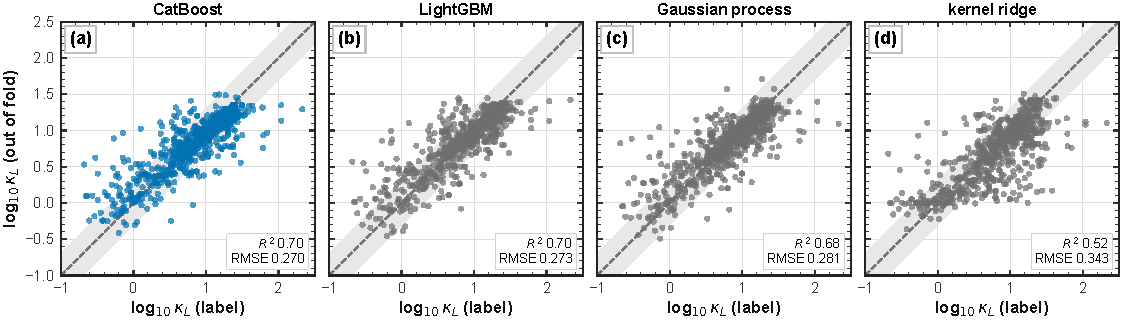
\includegraphics[width=\linewidth]{figures/fig13_parity_models.pdf}
  \caption{\textbf{Out-of-fold parity for the four regressors:} (a)~CatBoost (retained),
  (b)~LightGBM, (c)~Gaussian process, (d)~kernel ridge. Each was trained on the same \num{681} rows
  and scored on the same element-system folds. Each point is one row: predicted against label
  $\log_{10}\kappa_L$. Dashed line: parity; shading: a factor of two. Each panel prints $R^2$ and
  RMSE on $\log_{10}\kappa_L$; the text gives them unrounded. The labels are calculations, not
  measurements.}
  \label{fig:parity_models}
\end{figure*}

\begin{figure*}[tp]
  \centering
  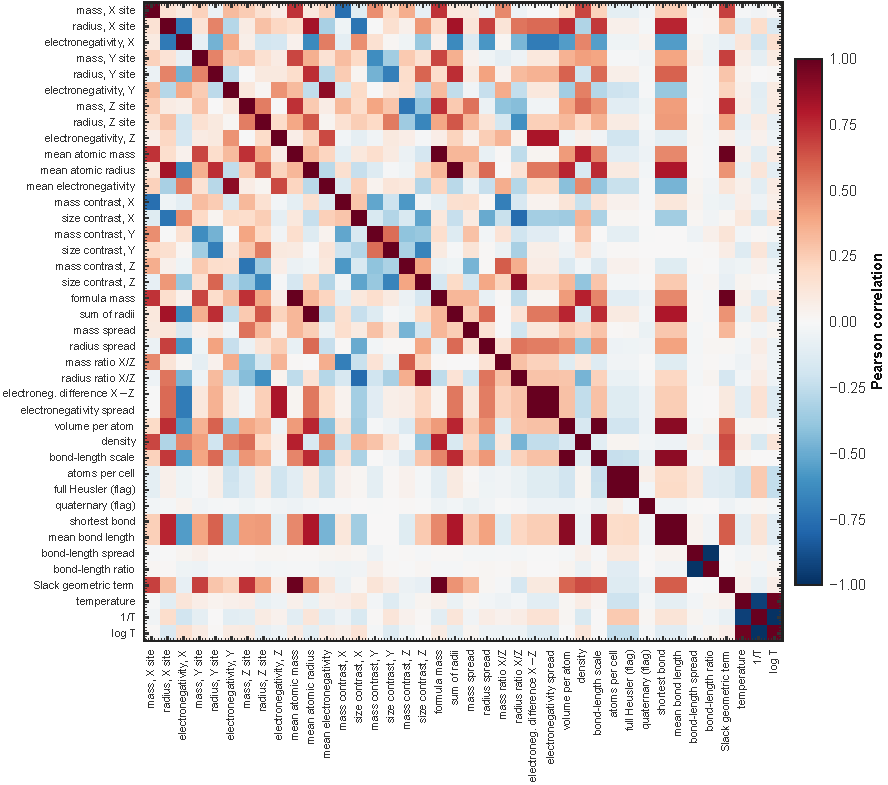
\includegraphics[width=\linewidth]{figures/fig14_feature_corr.pdf}
  \caption{\textbf{Correlation between the descriptors.} Pearson correlation over the training rows,
  for the model descriptors that vary across the pool. Each pair is computed over the rows on which
  both descriptors are defined, so rows without bond descriptors do not remove the others. The five
  disorder descriptors (zero on every row of this stoichiometric pool) are omitted. Dark off-diagonal
  squares mark nearly redundant pairs, which share attribution: for example, atoms per cell and the
  full-Heusler flag, shortest and mean bond length, and the three encodings of temperature.}
  \label{fig:feature_corr}
\end{figure*}

\begin{figure*}[tp]
  \centering
  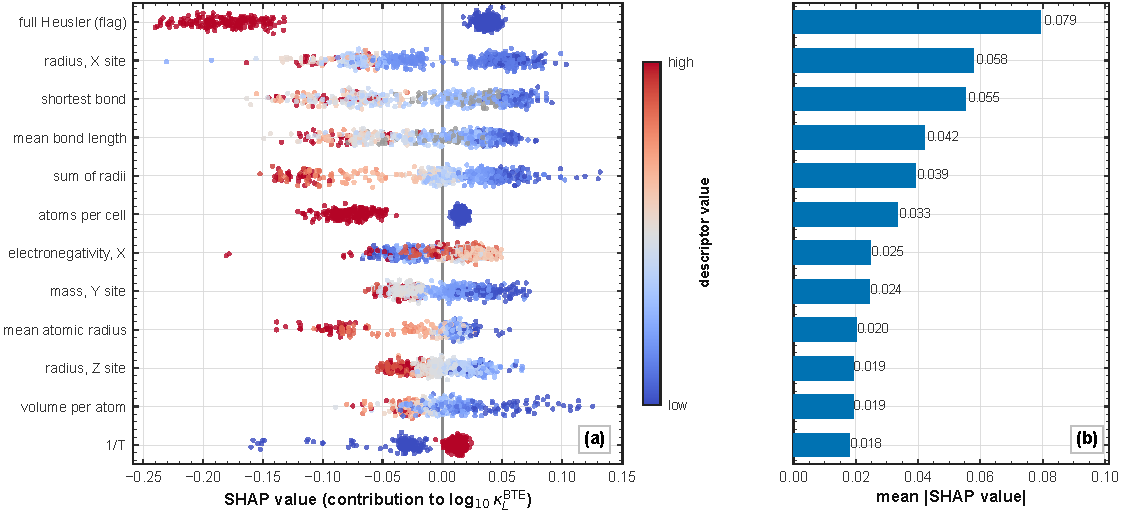
\includegraphics[width=\linewidth]{figures/fig11_shap.pdf}
  \caption{\textbf{What the machine-learning model has learned.} \textsc{shap} attribution of the
  reference-seed CatBoost model (\num{681} training rows) for the twelve of its \num{45}
  descriptors with the largest mean absolute contribution; the target is the calculation,
  $\log_{10}\kappa_L^{\mathrm{BTE}}$. (a)~Each point is one training row, placed at that
  descriptor's contribution and coloured by the descriptor's value (blue low, red high; grey where
  the bond descriptors are missing, \num{81} rows). (b)~Mean absolute contribution. Strongly
  correlated descriptors share their attribution.}
  \label{fig:shap}
\end{figure*}

\section{Accuracy above and below the cap temperature}
\label{sec:cap}

The shared and family transfer functions treat high temperature differently, and anyone applying
them should know where each stops correcting.

With $c=\num{0.42}$ and $p=\num{0.70}$, the shared form,
$\kappa_L^{\mathrm{BTE}}\min[c\,(T/300)^{p},1]$, reaches unity at \SI{1036}{\kelvin}. Above that
temperature, it returns the calculation unchanged. The cap is a modelling choice for the shared
route: it keeps a calibrated value from exceeding the calculation it starts from. In the main-text
offset comparison, \num{3} of the \num{189} matched calculation--measurement points lie above this
temperature. The blind test, the conditional estimates of Table~\ref{tab:conditional} and the
shared-constant estimates of Section~\ref{sec:structureonly} all use the capped form. Those estimates are all quoted at \SI{300}{\kelvin}, however, where the cap does not
bind.

The family form is uncapped: $\kappa_L^{\mathrm{BTE}}\,c_f\,(T/300)^{0.70}$. Family constants larger
than the shared one would reach a cap sooner, so we tested the choice where a cap would bind: on
rows where a family's own power law has passed unity. Of the \num{429} calculation--reference rows
scored with family constants, \num{60} lie there, on \num{12} compounds between \num{330} and
\SI{1080}{\kelvin}. On those rows, the uncapped form gives a median row error of
\SI{12.8}{\percent}, against \SI{24.6}{\percent} for the capped form (which, there, is the bare
calculation). The uncapped form is closer on \SI{58.0}{\percent} of rows. Five of the six families
prefer it; \ce{Co}--\ce{Bi}, on six rows, prefers the cap (Table~\ref{tab:cap}). The comparison is
per row and in sample, because the constants are fitted under the uncapped form. It therefore shows
that the uncapped form describes the measurements above the cap better, not that it predicts them
better.

The uncapped form has a cost that bears on validity. Unlike the shared form, it can exceed the
calculation: at the highest temperatures, a family value reaches \num{2.18} times the calculation.
There, the form describes measurements that lie above the calculation for the same compound. Above
the cap, the family form therefore describes what experiments report; it is not a correction with a
mechanism. Every issued value is quoted at \SI{300}{\kelvin}, or at \SI{500}{\kelvin} for three
compounds, and at those temperatures the family factor is below one for each.

\begin{table}[htb]
  \centering
  \caption{Median row error of the family form with and without the cap, on rows above their own
  family's cap temperature. Errors are per row. The constants are fitted under the uncapped form, so
  the comparison is in sample.}
  \label{tab:cap}
  \small
  \begin{tabular}{lccc}
    \toprule
    Family & Rows & Capped (\si{\percent}) & Uncapped (\si{\percent}) \\
    \midrule
    \ce{Bi}--\ce{Pd} & 24 & 28.0 & 11.2 \\
    \ce{Sn}--\ce{Pt} & 23 & 32.2 & 18.3 \\
    \ce{Co}--\ce{Bi} &  6 &  1.6 &  5.7 \\
    \ce{Ni}--\ce{Sb} &  3 & 21.8 & 19.5 \\
    \ce{Sb}--\ce{Pt} &  3 & 19.0 & 12.3 \\
    \ce{Ni}--\ce{Pb} &  1 & 11.6 &  5.0 \\
    \midrule
    All              & 60 & 24.6 & 12.8 \\
    \bottomrule
  \end{tabular}
\end{table}

\section{Cross-checking the extraction against an independent reading}
\label{sec:extraction}

An extracted value can be checked only where someone else has read the same paper. Three compounds
carry both our extraction and a Starrydata digitisation of the \emph{same} publication; on these,
the two readings differ by a median of \SI{0.6}{\percent}. That comparison rests on four matched
points, so it is a consistency check, not a validation. It is nonetheless the only direct check the
corpus supports, because extraction targeted publications that the curated database does not cover.
Comparing our readings against \emph{different} publications on the same compound gives a median
difference of \SI{8.7}{\percent}. That figure measures the spread between laboratories, not the
extraction. The largest single difference, a factor of \num{3.8} for \ce{NbFeSb}, is between
specimens, not readings.

\section{How far semi-empirical and transport values differ}
\label{sec:tiergap}

The main text keeps full transport calculations (tier~1) and semi-empirical estimates (tier~3) as
separate labels. Semi-empirical values never enter the calibration. In training, they appear only
for full Heuslers that have no calculation, and at reduced weight; half-Heusler semi-empirical
estimates are excluded from training. The corpus shows what that separation is worth. For the
\num{161} half Heuslers with both kinds of label in a matched \SI{100}{\kelvin} temperature bin
(\num{180} bins), the median disagreement is a factor of \num{1.25}, and \SI{90.1}{\percent} agree
within a factor of two. The tail, however, reaches \num{11.4} (\ce{HoSbPd}). A semi-empirical value
is usually close and occasionally very wrong, and nothing in the value itself shows which. So the
two cannot be averaged into one label.

\section{Predictions from crystal structure alone: further compounds}
\label{sec:structureonly}

The main text reports two compounds predicted from crystal structure alone, \ce{TmPbAu} and
\ce{HfTeOs}. This section gives the search they came from, the further estimates it yields, and the
evidence that limits each (Table~\ref{tab:structureonly}). Every value rests on two separately
validated steps: from structure to a theory-scale $\kappa_L$ (a value on the scale of the
first-principles calculation, $\kappa_L^{\mathrm{BTE}}$), and from theory scale to experiment. We
state their errors side by side and never combine them. From structure to theory scale, the model
reproduces published full calculations to a median \SI{21.9}{\percent}, with \SI{88.3}{\percent}
within a factor of two, over \num{230} compounds with \num{27} X-site clusters held out (one model
seed). From theory scale to experiment, the shared constant on families never measured gives a
median \SI{33.0}{\percent}, with \SI{79.4}{\percent} within a factor of two, over \num{34}
compounds. Where a compound's family has its own constant, we state that constant's held-out error
instead.

\subsection*{The search}

We collected candidates from public structure databases: DxMag~\cite{xiao2026accurate},
AFLOW~\cite{curtarolo2012aflow}, OQMD~\cite{kirklin2015the}, JARVIS~\cite{choudhary2020the} and the
Materials Project~\cite{jain2013commentary}. We kept compounds with 18 valence electrons, a cubic
$C1_b$ structure, and no published full transport calculation of $\kappa_L$. We searched for prior
work on each in OpenAlex~\cite{priem2022openalex}, Crossref and arXiv.

Before grading, we excluded any compound for which a structure database records a non-cubic
ordering lower in formation energy than the cubic cell, because the cubic phase it would describe may
not be the one that forms. Twenty-four compounds remain with no published value of $\kappa_L$ and no
other polymorph on record. We grade them by the support the model has for them. A compound is
\emph{strong} when, held out, the model reproduces the published calculations of its own family
members to a median error under \SI{25}{\percent}, and its five seeds agree closely. It is
\emph{moderate} when that family evidence or the seed agreement is weaker but still bounded. It is
\emph{weak} otherwise; its theory-scale value then cannot be trusted, and it is not quoted. Two are
strong (\ce{TmPbAu} and \ce{HfTeOs}, main text), none is moderate, and six are weak. A further
sixteen fill gaps in rare-earth series; they are graded weak because their lattice constants come
from the lanthanide contraction, not from a database cell. For \num{22} of the \num{24}, our search
of the three indices found no paper; one is named in papers that do not mention thermal
conductivity, and one was not checked.

A second group has a published $\kappa_L$ from a machine-learning surrogate (a model that stands in
for the first-principles calculation): the neural-network force field
Elemental-SDNNFF~\cite{rodriguez2023millionsca}. Of eleven such candidates, nine have no reported
first-principles or measured $\kappa_L$. Two of the nine are well supported: they contain neither
\ce{Zn} nor \ce{Cd}, have no non-cubic structure on record, and sit in families whose held-out
published calculations the model reproduces to better than \SI{25}{\percent}. The other seven fail
at least one of these conditions and are not quoted.

\subsection*{\ce{ZrTeOs} and \ce{ScBiPt}}

For these two, no first-principles or measured $\kappa_L$ has been reported, but a surrogate value
has been published. Our values are therefore, to our knowledge and within the search limits stated
above, the first estimates on the experimental scale; they are not the first estimates of
$\kappa_L$. At \SI{300}{\kelvin}, the model's theory-scale value for \ce{ZrTeOs} is
\SI{12.64}{\watt\per\meter\per\kelvin}, \num{0.85} times the surrogate's \num{14.86}. For
\ce{ScBiPt} it is \SI{6.76}{\watt\per\meter\per\kelvin}, \num{1.74} times the surrogate's
\num{3.89}. The five model seeds span a factor of \num{1.152} (\ce{ZrTeOs}) and \num{1.294}
(\ce{ScBiPt}). Held out, the model reproduces the published calculations of these families' members
to \SI{0.5}{\percent} for \ce{TiTeOs}, the one \ce{Te}--\ce{Os} member, and to a median
\SI{6.2}{\percent} for the nine \ce{Bi}--\ce{Pt} members. Neither family has a measured member, so we
place both on the experimental scale with the shared constant: \SI{5.31}{\watt\per\meter\per\kelvin}
for \ce{ZrTeOs} and \SI{2.84}{\watt\per\meter\per\kelvin} for \ce{ScBiPt}. The surrogate value for
\ce{ZrTeOs} is also the input to the main-text \ce{HfTeOs} cross-check. Side by side, the errors are
\SI{21.9}{\percent} for the model step, and a median \SI{33.0}{\percent} (\SI{79.4}{\percent} within
a factor of two) for the shared constant on families never measured.

Chemical twins are compounds that differ only by an element and its heavier congener (\ce{Zr} and
\ce{Hf}, \ce{Nb} and \ce{Ta}, \ce{Ru} and \ce{Os}, \ce{Pd} and \ce{Pt}). A model-free relation
between twins serves as a cross-check only. Estimating each member of \num{23} twin pairs from the
other with a flat ratio gives a median error of \SI{12.2}{\percent}, against \SI{9.8}{\percent} for
the model on the same pairs. We therefore do not use it as a prediction route.

\subsection*{\ce{LuSbPd} and \ce{SmBiPd}: flagged}

Two compounds sit inside calibrated families and have no published $\kappa_L$, but they are flagged
rather than issued; we record their values here as flagged values only. In both, the lattice
constant comes from the rare-earth contraction across the family's training lattices (four
\ce{Sb}--\ce{Pd} and nine \ce{Bi}--\ce{Pd} compounds), not from a database cell.

\ce{LuSbPd} is flagged because its family fails held out. The \ce{Sb}--\ce{Pd} constant
($c_f=\num{0.24}$) predicts the family's own members to \SI{61.5}{\percent}, far outside the
\SI{25}{\percent} threshold; this is also why \ce{TmSbPd} is flagged in the main text. At
\SI{300}{\kelvin}, the model gives \SI{7.66}{\watt\per\meter\per\kelvin} on the theory scale, with
seeds spanning a factor of \num{1.124}. With the family constant this becomes
\SI{1.84}{\watt\per\meter\per\kelvin} (\SI{50}{\percent} band \numrange{1.14}{2.98},
\SI{90}{\percent} band \numrange{0.65}{5.24}). That is a factor of \num{1.08} below the
\SIrange{1.98}{3.60}{\watt\per\meter\per\kelvin} span of the measured \ce{Sb}--\ce{Pd} compounds.
Extending the published calculations along the rare-earth series gives \num{7.64} on the theory
scale and \SI{1.83}{\watt\per\meter\per\kelvin} with the family constant, so the two routes agree
(ratio \num{1.00}). The model is sound on lutetium: with each of seven lutetium compounds held out,
its error is \SIrange{2.8}{14.9}{\percent}. The step that fails is the calibration.

\ce{SmBiPd} is flagged for two reasons. First, samarium is valence-fluctuating, so the
valence-electron count of \ce{SmBiPd} is not secure at 18. Second, its family, \ce{Bi}--\ce{Pd}
($c_f=\num{0.95}$), predicts its own members to \SI{25.3}{\percent} held out, just outside the
threshold. At \SI{300}{\kelvin}, the model gives \SI{5.14}{\watt\per\meter\per\kelvin} on the theory
scale, with seeds spanning a factor of \num{1.155}. With the family constant this becomes
\SI{4.88}{\watt\per\meter\per\kelvin} (\SI{50}{\percent} band \numrange{3.01}{7.91},
\SI{90}{\percent} band \numrange{1.71}{13.91}). That is a factor of \num{1.38} above the
\SIrange{3.17}{3.53}{\watt\per\meter\per\kelvin} span of the measured \ce{Bi}--\ce{Pd} compounds, a
clear extrapolation. Interpolating the published calculations along the rare-earth series gives
\num{5.53} on the theory scale and \SI{5.25}{\watt\per\meter\per\kelvin} with the family constant;
the ratio of the two routes is \num{0.93}. The model is uneven on samarium: with each samarium
compound among its calculated labels held out, its errors on \ce{SmNiBi}, \ce{SmOF} (an oxyfluoride
of the training pool, not a half Heusler) and \ce{SmSnAu} are \SI{18.6}{\percent},
\SI{1.0}{\percent} and \SI{46.0}{\percent}.

For both, the errors side by side are \SI{21.9}{\percent} for the model step against published
calculations, and \SI{61.5}{\percent} (\ce{Sb}--\ce{Pd}) and \SI{25.3}{\percent} (\ce{Bi}--\ce{Pd})
for the family constants held out. The bands are the main-text conformal bands; their coverage is
not validated for a family that fails held out.

\begin{table}[htb]
  \centering
  \caption{Further estimates from crystal structure alone, at \SI{300}{\kelvin}. \emph{Theory
  scale}: regression-model value, with the factor spanned by its five seeds in brackets.
  \emph{Surrogate}: the published Elemental-SDNNFF value~\cite{rodriguez2023millionsca}. Errors of
  the two steps, never combined: (i)~model against published calculations, \SI{21.9}{\percent}
  median, \SI{88.3}{\percent} within $2\times$ (\num{230} compounds, \num{27} X-site clusters held
  out, one seed); (ii)~shared constant on families never measured, \SI{33.0}{\percent} median,
  \SI{79.4}{\percent} within $2\times$ (\num{34} compounds); (iii)~family constants held out,
  \SI{61.5}{\percent} (\ce{Sb}--\ce{Pd}) and \SI{25.3}{\percent} (\ce{Bi}--\ce{Pd}).}
  \label{tab:structureonly}
  \small
  \setlength{\tabcolsep}{3pt}
  \resizebox{\linewidth}{!}{%
  \begin{tabular}{llllcll}
    \toprule
    Compound & Family & Theory scale & Surrogate & Calibration & Experimental scale & Status \\
    & & \multicolumn{2}{c}{(\si{\watt\per\meter\per\kelvin})} & & (\si{\watt\per\meter\per\kelvin}) & \\
    \midrule
    \ce{ZrTeOs} & \ce{Te}--\ce{Os} & 12.64 ($\times$1.152) & 14.86 & shared & 5.31 & estimate$^{a}$ \\
    \ce{ScBiPt} & \ce{Bi}--\ce{Pt} & 6.76 ($\times$1.294)  & 3.89  & shared & 2.84 & estimate$^{a}$ \\
    \ce{LuSbPd} & \ce{Sb}--\ce{Pd} & 7.66 ($\times$1.124)  & ---   & family & 1.84 & flagged$^{b}$ \\
    \ce{SmBiPd} & \ce{Bi}--\ce{Pd} & 5.14 ($\times$1.155)  & ---   & family & 4.88 & flagged$^{c}$ \\
    \bottomrule
  \end{tabular}}

  \vspace{2pt}
  \begin{minipage}{\linewidth}\footnotesize
    $^{a}$ No first-principles or measured $\kappa_L$ has been reported; a surrogate value has
    been published.\par
    $^{b}$ The \ce{Sb}--\ce{Pd} family constant fails held out (\SI{61.5}{\percent}).\par
    $^{c}$ Samarium is valence-fluctuating, so $\mathrm{VEC}=18$ is an assumption. The
    \ce{Bi}--\ce{Pd} family constant misses the \SI{25}{\percent} threshold held out
    (\SI{25.3}{\percent}). The value lies above the family's measured range.
  \end{minipage}
\end{table}

% ---------------------------------------------------------------------------------------------
% S12 EXTENDED METHODS and S13 FLAGGED COMPOUNDS -- moved from the main text in the 2026-10-05
% condensing pass. Appended after S11 so that the section numbers the main text quotes (S3) do not
% move. Numbers are those of the main text, from paper_numbers.json / PAPER_PREDICTIONS.csv:
%   1036 K, 0.42, 0.70, 0.58, 1.21, 0.45-1.15   calibration.*; 1 - c; p/(1 - c)
%   -1.02 slope                                  carry_exponent (the one tier-1 curve at >= 3 T)
%   0.946, 23 pairs, 12.2 vs 9.8                 twin_estimates
%   681 / 463 / 284 / 230; 0.21 / 213.5 / 7.57;  training_data.*
%     544 / 119
%   populations 735/284/50/39/11/34/31/22         corpus.*, blind_test, offset, deployed_route,
%                                                in_domain_table.published_semi_empirical
%   flagged table                                PAPER_PREDICTIONS.csv (status FLAGGED, margins)
% ---------------------------------------------------------------------------------------------

\section{Extended Methods}
\label{sec:extmethods}

This section gives in full the rules that the main-text Methods state in outline. Section and
equation names refer to the main text.

\subsection*{Corpus curation rules}

\emph{Extraction gate.} When the body text of an article is unavailable, a publisher's full-text
service may return only a metadata record (title, identifiers and references). Such a record
contains no measurement, so extraction is gated on content, not on size: a retrieved record with no
body text (no paragraph or section elements) is never passed to the language model, and any value
attributed to such a record is excluded from every analysis. Some compounds enter the corpus only
through direct extraction; they include three of the four measured members of the \ce{Sb}--\ce{Pt}
family (\ce{DySbPt}, \ce{LuSbPt}, \ce{TbSbPt}), a family in which predictions are issued.

\emph{Separating the lattice term.} The Lorenz number of the Wiedemann--Franz subtraction is
$L = 1.5 + \exp(-|S|/116)$, in units of \SI{1e-8}{\watt\ohm\per\kelvin\squared}, with the Seebeck
coefficient $S$ in \si{\micro\volt\per\kelvin}~\cite{kim2015characteri}. The remaining measured rows
take one of three routes: $L$ at the degenerate limit, \SI{2.44e-8}{\watt\ohm\per\kelvin\squared};
subtraction of an independently measured electronic term; or a lattice conductivity published
directly. We require the resistivity to lie between \SI{1e-8}{\ohm\meter} and \SI{1e-2}{\ohm\meter}.
If a row carries a resistivity of order \SI{10}{\ohm\meter}, $LT/\rho$ falls to zero, the
subtraction removes nothing, and the row reports the \emph{total} conductivity under a lattice
label; the signature of this silent failure is an apparent lattice conductivity that rises with
temperature. Among others, this gate removes every measured row of \ce{TiCoSn}.

\emph{What counts as a measurement.} Four rules, each applied in code when the corpus is generated:
\begin{enumerate}
  \item \emph{A value one paper quotes from another is not a measurement.} Computational papers often
        place a literature value beside their own result, and an extraction can file it as the
        paper's own. We read every source that carries a measured row and meets any one of three
        criteria: it is also a source of calculated rows; it has a computational title; or it adds two
        or fewer rows to a compound measured by three or more other sources. If such a source only
        quotes the value, its measured rows are removed; its calculated rows are kept.
  \item \emph{One copy per sample.} Starrydata can digitise one sample twice: as the authors'
        published lattice curve, and as the total-conductivity curve from which a second lattice
        value is derived by Wiedemann--Franz subtraction. Where a sample has a published lattice
        curve, the derived copy is dropped.
  \item \emph{A data deposit is not a laboratory.} A deposit row that matches a row from a primary
        publication (same compound, within \SI{1}{\kelvin} and \SI{1}{\percent}) is a copy and is
        dropped; the other deposit rows are kept, but a deposit never counts as a laboratory and
        ranks below every laboratory when a reference is chosen.
  \item \emph{A composition must be a Heusler.} Compositions that pass the formula-ratio test but are
        not Heuslers (a two-phase composite, ternary oxides, a rocksalt chalcogenide) are named in
        code and removed. Real compounds outside the cubic structure are kept at this stage; the
        structural screen of the domain excludes them later.
\end{enumerate}

\emph{Identity of calculations.} Provenance is keyed on DOI, and an arXiv preprint or a data deposit
carries a different identifier from the article it duplicates, so one calculation could be counted
as two independent groups. Because a paper agrees with itself exactly, each such pair would pull any
between-source spread statistic toward a ratio of one. Every pair of sources sharing three or more
compounds is therefore tested for identical values, which two independent calculations do not
produce, and a matching pair is collapsed onto its version of record.

\subsection*{The reference-choice ladder}

When several groups have measured a compound, a fixed ladder chooses one laboratory as the
reference. It reads only the specimen and the temperature coverage of each measurement, never a
calculation or a model value. The first rung that applies decides:
\begin{enumerate}
  \item If four or more laboratories report the compound (data deposits not counted), choose the
        central one: the laboratory closest, in logarithm, to the median of their curves.
  \item Otherwise, among sources that report a relative density, choose the densest specimen,
        breaking ties first in favour of a single-phase specimen, then the widest temperature range.
  \item Otherwise, among sources whose full text we hold, whose samples were recorded and whose
        stored text has been verified to be that publication, choose the widest temperature range.
  \item Otherwise, choose the source nearest the logarithmic median of all sources for that
        compound.
\end{enumerate}
Remaining ties break to the widest range and then by DOI, so the choice is deterministic.

\emph{The family-paper rung.} A family constant describes one kind of specimen, and members referenced
to different laboratories mix kinds of specimen. The rung applies when one primary publication (not a
data deposit) has measured two or more members of a family; only members it reports at four or more
temperatures, on a specimen that is not nanostructured, count. That publication then becomes the
reference for every member it covers that fewer than four laboratories have measured; a member
measured by four or more keeps the central laboratory. If several publications qualify we choose, in
order, the one covering the most members, then one whose full text we hold, then the one with the
most recorded densities, then the widest temperature span.

\emph{Sources ranked last.} Four kinds of source rank below every alternative at each rung. They are
never deleted: where such a source is a compound's only measurement it remains the reference, and the
record says so.
\begin{enumerate}
  \item \emph{A laboratory that contradicts a consensus.} On any compound measured near
        \SI{300}{\kelvin} by four or more sources, a source more than a factor of two from the
        geometric mean of the others is ranked last for every compound it reports. A Lorenz number
        wrong by a constant factor leaves a curve's shape intact, so this is the only test the corpus
        can make for such an error.
  \item \emph{A data deposit}, which republishes curves already in the corpus.
  \item \emph{A nanostructured specimen}: ball-milled for \SI{10}{\hour} or longer, a reported grain
        size below \SI{1}{\micro\metre}, a synthesis record that describes it as nanostructured, or a
        title that names a nanostructuring process. A reported grain size decides for all of a
        publication's specimens and milling time is then not consulted, since long milling that
        leaves micrometre grains is powder preparation, not grain refinement. The calculation
        describes a bulk crystal and grain refinement is the standard route to a suppressed lattice
        conductivity, so such a specimen is a deliberate departure from what is calibrated. It
        remains the reference where nothing else exists, as for \ce{TaCoSn} and \ce{ZrNiPb}, both
        measured only on specimens ball-milled for \SI{20}{\hour}.
  \item \emph{A source reporting fewer than four temperatures}, since a temperature-dependent
        calibration cannot be scored against a point.
\end{enumerate}

\emph{Curve shape.} Lattice conduction falls with temperature, as $T^{-1}$ where Umklapp scattering
dominates and more slowly when extrinsic scattering is added. A measured curve of four or more
points is rejected if it rises faster than $T^{+0.2}$ over at least \SI{150}{\kelvin} (electronic term
under-subtracted) or falls more steeply than $T^{-2}$ (over-subtracted). In the blind test, a compound
whose every curve fails this test keeps its measurement, ranked last and recorded as such, so the
scored population does not depend on this gate.

\emph{Where the reference is used.} The single reference is used in the shared and family constants,
the blind test, the null baselines, the prediction intervals and every table. The family-paper rung
is dropped in two places so that a scored compound's reference never depends on which of its
siblings have been measured: in the blind test every compound is referenced without it, and in the
leave-one-compound-out family test references are re-chosen inside each fold, the held-out compound
being referenced without the rung and not counted as a member when its siblings' family publication
is chosen.

\subsection*{Method tiers and quality-control gates}

The tier is assigned from the method string, never from a repository's own label, and tier~1 requires
a positive match for a transport solution with no disclaimer attached. Many half-Heusler records
carry a method string that names the Boltzmann transport equation while disclaiming a full solution
(``reduced model'', ``\textsc{bte}-approx'', ``not full \textsc{bte}''); a keyword match would admit
each as first-principles. A dataset whose coarse label reads ``\textsc{bte}'' but whose documentation
names machine-learned force constants is tier~2. Section~\ref{sec:tiergap} compares tier-1 and tier-3
values for compounds that carry both.

Five further conditions are applied when the corpus is generated. A value that fails condition 1, 3,
4 or 5 is excluded from every analysis; condition 2 marks a compound, and the domain acts on the mark.
\begin{enumerate}
  \item \emph{Cubic record.} A compound is admitted as a half Heusler only if a cubic $C1_b$ record
        (space group 216) exists in a source that is not a prototype-substitution database, since a
        prototype decoration records that a structure was generated, not that the phase forms.
  \item \emph{Polymorph flag.} A compound also recorded in a non-cubic space group is flagged as
        polymorphic, for example \ce{MgAgSb} (space groups 129 and 216) and \ce{DySbPd} (186, 194 and
        216).
  \item \emph{Half versus full Heusler,} separated by the measured site ratio, not by how the formula
        looks; a binary in space group 225 is fluorite, not a Heusler.
  \item \emph{Temperature floor.} Values below \SI{200}{\kelvin} are excluded. As $T\to 0$ Umklapp
        scattering freezes out and the boundary-free calculated conductivity diverges, whereas the
        measurement becomes boundary-limited and specific to the specimen.
  \item \emph{Method string.} A tier-1 row must carry a transport-calculation method string, not a
        semi-empirical one.
\end{enumerate}

\subsection*{Compound populations}

Several sub-populations recur in the main text. Accuracy figures over different rows of
Table~\ref{tab:populations} are not directly comparable; this matters most when the family constants
are set against the shared constant, which is done only on the \num{31}.

\begin{table}[htb]
  \centering
  \caption{The compound populations used in the main text.}
  \label{tab:populations}
  \small
  \begin{tabular}{clp{0.55\linewidth}}
    \toprule
    $n$ & name & definition \\
    \midrule
    \num{735} & half-Heusler corpus & any thermal-conductivity record of any kind \\
    \num{284} & calculated & carries a full Boltzmann-transport calculation (tier~1) \\
    \num{50}  & measured & measured in a laboratory; every one is scored in the blind test \\
    \midrule
    \num{39}  & \textbf{in-domain} & the \num{50} inside the domain of applicability;
                \textbf{the population behind the headline figure} \\
    \num{11}  & excluded & the remainder of the \num{50}, scored separately \\
    \midrule
    \num{34}  & published route & in-domain compounds whose published calculation can be paired with
                their reference; the population of the offset, of the shared-constant fit and of
                the deployed route \\
    \num{31}  & family held out & of the \num{34}, those in a family with at least one other measured
                member, each predicted with its own measurement withheld \\
    \num{22}  & semi-empirically covered & in-domain compounds carrying a published Slack or
                Debye--Callaway estimate \\
    \bottomrule
  \end{tabular}
\end{table}

\subsection*{Training data of the machine-learning model}

Figure~\ref{fig:dataset} shows the distribution of the \num{681} training labels on \num{463}
compounds. The label values span \SIrange{0.21}{213.5}{\watt\per\meter\per\kelvin}, with a median of
\SI{7.57}{\watt\per\meter\per\kelvin}; the distribution is strongly right-skewed, so the model is
fitted on $\log_{10}\kappa_L^{\mathrm{BTE}}$, on which it is far closer to symmetric. The descriptors
order the elements by electronegativity (most electropositive on X, most electronegative on Z), which
can differ from the chemical labels of the site convention: in the \ce{Sb}--\ce{Pt} compounds it
places \ce{Pt} on Z. The bond descriptors require atomic coordinates; a half Heusler being predicted
whose record lacks them receives the ideal $C1_b$ positions, so its bond descriptors depend on the
lattice parameter alone. Lattice parameters must be reduced to one convention before use, because some
sources publish the edge of the primitive face-centred cell and others the conventional cubic cell
($a_\mathrm{conv} = \sqrt{2}\,a_\mathrm{prim}$); mixing them injects a \SI{41}{\percent} error into
every length descriptor and \SI{183}{\percent} into volume-derived ones, which is why the lattice
parameter itself is never a descriptor.

\begin{figure*}[tp]
  \centering
  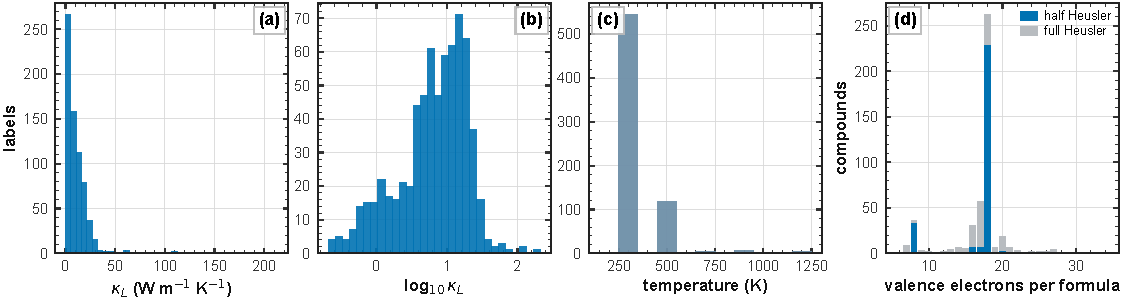
\includegraphics[width=\linewidth]{figures/fig12_dataset.pdf}
  \caption{\textbf{The training data of the machine-learning model.} \num{681} labels of
  $\kappa_L^{\mathrm{BTE}}$ on \num{463} compounds; every half-Heusler label is a full
  first-principles Boltzmann-transport calculation. (a)~The labels on a linear scale, from
  \num{0.21} to \SI{213.5}{\watt\per\meter\per\kelvin} (median \num{7.57}): the distribution is
  strongly skewed, so the model is fitted on $\log_{10}\kappa_L$, shown in (b). (c)~Temperatures of
  the labels: \num{544} at \SI{300}{\kelvin} and \num{119} at \SI{500}{\kelvin}, the few others
  spread up to \SI{1200}{\kelvin}, so the temperature dependence is only weakly constrained by the
  training data. (d)~Compounds by valence-electron count per formula unit: \num{284} half Heuslers
  (blue), \num{230} of them at 18, and full Heuslers (grey), which share the descriptors and enter
  the pool beside them.}
  \label{fig:dataset}
\end{figure*}

\subsection*{Pairing a calculation with a measurement}

A published calculation is usually a single value at \SI{300}{\kelvin}, whereas a measurement is a
curve. Pairing follows four rules:
\begin{enumerate}
  \item A calculation reported at two or more temperatures is interpolated between them in log--log
        space, which reproduces whatever power law it actually follows.
  \item A calculation reported at one temperature is carried to the measurement temperature as
        $\kappa_L^{\mathrm{BTE}} \propto 1/T$, the high-temperature limit of three-phonon Umklapp
        scattering. The one tier-1 published curve in the corpus reported at three or more
        temperatures has a log--log slope of \num{-1.02}.
  \item No value is carried by more than a factor of \num{2.5} in temperature in either direction,
        and none below \SI{200}{\kelvin}. A measurement with no calculation reachable under this rule
        contributes no pair.
  \item Where independent calculations exist, the calculated value at each temperature is their
        median. A temperature at which they disagree by more than a factor of two is
        \emph{contested} and contributes no pair, since the median of two numbers that far apart is
        not a calculation. A compound whose every calculated temperature is contested keeps the
        single calculation closest to the median of its family-mates' uncontested calculations.
\end{enumerate}
The same rules apply to prediction candidates: a contested temperature is not used and the
prediction is quoted from the uncontested calculation. The rules compare calculations only with
calculations and never read a measurement.

\subsection*{Why the correction is not a boundary-scattering term}

In a Callaway grey-boundary treatment~\cite{callaway1959model} with a single boundary length
$\Lambda_\mathrm{b}$, the suppression factor is $S = \Lambda_\mathrm{b}/(\Lambda+\Lambda_\mathrm{b})$,
where $\Lambda$ is the intrinsic phonon mean free path. For $\Lambda \propto 1/T$, the logarithmic
slope of $S$ at \SI{300}{\kelvin} is $1-S$, so a model that reproduces $S(300)=c$ must have $p = 1-c$.
Allowing a per-mode suppression $S_\omega$ and any distribution of mode conductivities, the slope
becomes $1 - \langle S^2\rangle_\kappa/\langle S\rangle_\kappa$, which by the Cauchy--Schwarz
inequality is at most $1-\bar S$, with $\bar S = \langle S\rangle_\kappa$ the conductivity-weighted
mean suppression. No single-boundary-length model, grey or spectral, therefore gives a slope above
$1-c$. At $c=\num{0.42}$ that ceiling is \num{0.58}; the fitted $p=\num{0.70}$ lies above it by a
factor of \num{1.21}. The bootstrap range of $p$ (\numrange{0.45}{1.15}) straddles the ceiling, so the
data can neither confirm nor exclude a single-boundary-length picture, and the transfer functions are
empirical, with no mechanism attached to their parameters.

\subsection*{The structure-only search procedure}

\emph{Candidates and structures.} We searched DxMag~\cite{xiao2026accurate},
AFLOW~\cite{curtarolo2012aflow}, OQMD~\cite{kirklin2015the}, JARVIS~\cite{choudhary2020the} and the
Materials Project~\cite{jain2013commentary}, through OPTIMADE~\cite{andersen2021optimade} where
available, for cubic $F\bar{4}3m$ 1:1:1 cells with the $C1_b$ arrangement (space group 216), checked on
the cell itself where the database does not state it, and kept only compounds inside the domain. A
half Heusler can be stored in three orderings, depending on which element occupies the tetrahedral
site, and their lattice parameters differ by a few per cent; because the bond descriptors are
computed on ideal positions, the ordering reaches the model only through the lattice parameter. We
take the lattice parameter from the first of: (1)~the cubic ordering of lowest formation energy,
where OQMD or AFLOW energies were retrieved; (2)~the DxMag cubic row of lowest hull distance, never a
row more than \SI{0.3}{\electronvolt} per atom above the hull, which marks a wrong site ordering;
(3)~the JARVIS cubic entry of lowest formation energy; (4)~otherwise, an ordering rule checked on
training compounds of known lattice parameter (the smallest of the orderings for a transition-metal
or rare-earth X site, their median for an alkali or alkaline-earth X site). Where a rare-earth
compound's only database cell has a wrong ordering, we interpolate its lattice parameter along the
lanthanide contraction of its family's training members.

\emph{Chemistry the model may reach.} A candidate is predicted only if (a)~its bonding family
contains at least one training half Heusler; (b)~its X element sits on the X site of at least three
training half Heuslers and belongs to a class (transition metal, rare earth, or alkali and alkaline
earth) seen on the X site of that family; (c)~every element appears in at least five training half
Heuslers; and (d)~no element is radioactive or valence-fluctuating.

\emph{The literature check.} Each candidate is checked against every thermal-conductivity dataset we
hold; against published machine-learning surrogate values~\cite{rodriguez2023millionsca}, checked
separately; and against the literature in OpenAlex~\cite{priem2022openalex}, Crossref and arXiv. A
paper counts as naming a compound only if the formula, in any element order, appears exactly in the
title or abstract (OpenAlex also searches full text where it holds it). \ce{ZrNiSn} is the positive
control for every index, and if an index fails to return, the compound is left unresolved, never
recorded as ``no paper found''. Each candidate is placed on a three-rung ladder: (1)~no published
report of any kind; (2)~calculated, but $\kappa_L$ never reported; or (3)~only a machine-learning
surrogate value exists. In case~(3) our value is, to our knowledge and within the limits of this
search, the first estimate on the experimental scale, and it is not described as novel.

\emph{Model-free cross-checks.} Two estimates use no machine learning and serve only as cross-checks.
The first interpolates a rare-earth series: the published \SI{300}{\kelvin} calculations of a
family's trivalent lanthanide members are fitted linearly in atomic number, excluding \ce{Sc},
\ce{Y} and \ce{La}; the fit is an extrapolation when the target lies beyond the end of the series.
The second takes a 5d compound's $\kappa_L^{\mathrm{BTE}}$ as its 4d twin's calculated value
(\ce{Zr}/\ce{Hf}, \ce{Pd}/\ce{Pt} and the like) times a single ratio, \num{0.946}. Fitted
leave-one-out over \num{23} pairs of calculated values, this ratio reproduces the held-out member to a
median \SI{12.2}{\percent}, against \SI{9.8}{\percent} for the model on the same pairs, so it does not
outperform the model.

\section{Flagged compounds and the full prediction landscape}
\label{sec:flagged}

Table~\ref{tab:refusals} lists the fifteen compounds that carry a calibrated value but are declined,
with the value and the condition each fails; the main text discusses them. Figure~\ref{fig:landscape}
sets out everything the method can say from a published calculation under the three prediction
statuses. The range gate behind the marginal and clear extrapolations is a conservative choice, not a
validated filter: marginal cases are issued because held-out measured compounds just outside their
family's span were predicted about as well as those inside it, and the margins are listed so that
each case can be weighed.

% [!htbp] here and below: at [htb] a float too tall for a top or bottom slot could only wait for the
% closing \clearpage, holding every later float behind it and leaving near-empty pages at the end.
\begin{table}[!htbp]
  \centering
  \caption{The fifteen flagged compounds: each carries a calibrated value but is declined, with the
  value and the condition it fails. A margin is the factor by which the value falls beyond the
  nearest edge of the family's measured span at \SI{300}{\kelvin}; a margin under \num{1.33}, the
  median disagreement between laboratories, is marginal. The \ce{Bi}--\ce{Pd} span is set by the two
  \ce{Bi}--\ce{Pd} compounds measured near room temperature. The two \ce{Sb}--\ce{Ir} values are
  quoted at \SI{500}{\kelvin}, the temperature of their only calculation.}
  \label{tab:refusals}
  \small
  \setlength{\tabcolsep}{4pt}
  \begin{tabular}{llccp{0.42\linewidth}}
    \toprule
    Compound & Family & $T$ & value & Condition failed \\
    & & (\si{\kelvin}) & (\si{\watt\per\meter\per\kelvin}) & \\
    \midrule
    \ce{DyBiPd} & \ce{Bi}--\ce{Pd} & 300 & 6.58 & family fails (\SI{25.3}{\percent} held out); \num{1.86} above the measured ceiling \\
    \ce{TbBiPd} & \ce{Bi}--\ce{Pd} & 300 & 6.58 & family fails; \num{1.86} above the ceiling \\
    \ce{HoBiPd} & \ce{Bi}--\ce{Pd} & 300 & 6.44 & family fails; \num{1.82} above the ceiling \\
    \ce{TmBiPd} & \ce{Bi}--\ce{Pd} & 300 & 5.97 & family fails; \num{1.69} above the ceiling \\
    \ce{ScBiPd} & \ce{Bi}--\ce{Pd} & 300 & 5.56 & family fails; \num{1.57} above the ceiling \\
    \ce{LuBiPd} & \ce{Bi}--\ce{Pd} & 300 & 5.46 & family fails; \num{1.55} above the ceiling \\
    \ce{NdBiPd} & \ce{Bi}--\ce{Pd} & 300 & 4.80 & family fails; \num{1.36} above the ceiling \\
    \ce{YBiPd}  & \ce{Bi}--\ce{Pd} & 300 & 4.03 & family fails; marginal, \num{1.14} above the ceiling \\
    \ce{PrBiPd} & \ce{Bi}--\ce{Pd} & 300 & 3.98 & family fails; marginal, \num{1.13} above the ceiling \\
    \ce{TmSbPd} & \ce{Sb}--\ce{Pd} & 300 & 1.84 & family fails (\SI{61.5}{\percent} held out); marginal, \num{1.08} below the floor \\
    \ce{DySbPd} & \ce{Sb}--\ce{Pd} & 300 & 1.84 & polymorphic: space groups 186 and 194 recorded beside 216; family fails \\
    \ce{LaSbPt} & \ce{Sb}--\ce{Pt} & 300 & 1.05 & \num{2.00} below the measured \ce{Sb}--\ce{Pt} floor \\
    \ce{ScSbPt} & \ce{Sb}--\ce{Pt} & 300 & 7.50 & \num{1.97} above the measured \ce{Sb}--\ce{Pt} ceiling \\
    \ce{HfSbIr} & \ce{Sb}--\ce{Ir} & 500 & 3.86 & family fails: its anchored constant misses its one member by \SI{36.6}{\percent} \\
    \ce{TiSbIr} & \ce{Sb}--\ce{Ir} & 500 & 3.60 & family fails, as above \\
    \bottomrule
  \end{tabular}
\end{table}

\begin{figure*}[tp]
  \centering
  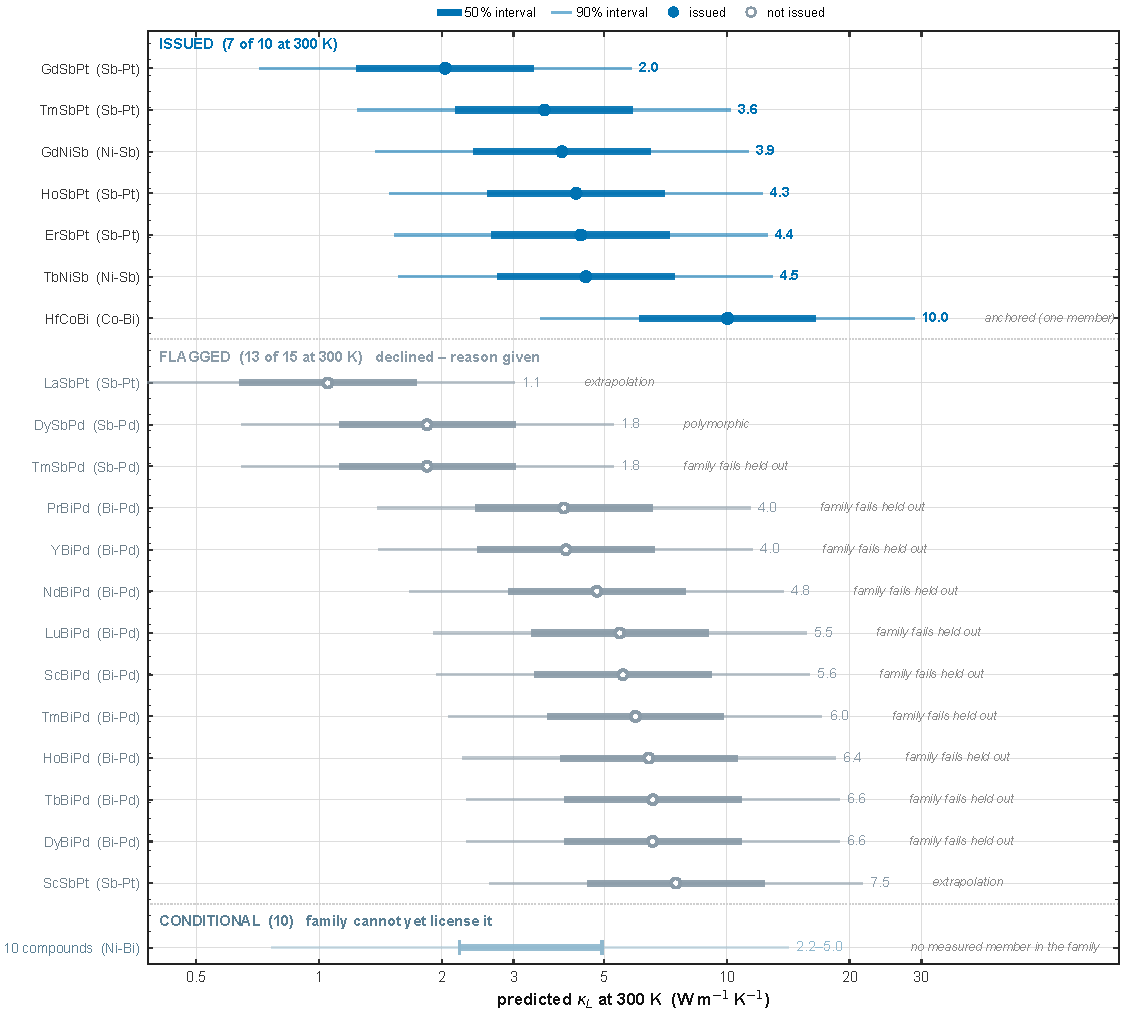
\includegraphics[width=\linewidth]{figures/fig06_landscape.pdf}
  \caption{\textbf{Everything the method can say from a published calculation, and what each
  statement is worth.} The three prediction statuses, ordered by the evidence behind them, on a
  \SI{300}{\kelvin} axis. \textsc{Issued} holds the issued predictions of the main text (seven of
  the ten are quoted at \SI{300}{\kelvin}), the one resting on a single measured compound marked as
  anchored. \textsc{Flagged} holds the compounds of Table~\ref{tab:refusals} (thirteen of the
  fifteen at \SI{300}{\kelvin}), which carry a calibrated value but fail one further check, named
  beside each. \textsc{Conditional} holds the ten \ce{Ni}--\ce{Bi} estimates on the shared constant
  (Table~\ref{tab:conditional}), whose family has no usable measured member; because they make a
  single statement they are drawn as one bracket spanning their values. Compounds quoted at
  \SI{500}{\kelvin} (three issued: \ce{TiCoBi}, \ce{HfNiPb}, \ce{TiNiPb}; two flagged: \ce{HfSbIr},
  \ce{TiSbIr}) are off this room-temperature axis and are given in the tables. Bars are the
  \SI{50}{\percent} and \SI{90}{\percent} conformal intervals; they do not widen from one status to
  the next, and for the conditional estimates, on the shared constant in a family never measured,
  their coverage is not validated. Only issued predictions carry a filled marker.}
  \label{fig:landscape}
\end{figure*}

\section{Families calibrated but not validated held out}
\label{sec:famcalsupp}

Table~\ref{tab:famcalsupp} gives the held-out test for the four families with two or more members
whose held-out median error is \SI{25}{\percent} or more, and for \ce{Sb}--\ce{Ir}, whose single
member is not reproduced within that bar even in sample. Each compound is predicted from its
family-mates alone, with the references re-chosen inside the fold, exactly as for the validated
families of the main text. Fitted on its own reference paper, each of the four reproduces its members
to \SIrange{2.8}{7.3}{\percent}; the constant does not transfer from one member to the next because
the members differ as materials. None of the five families issues a prediction: the \ce{Bi}--\ce{Pd},
\ce{Sb}--\ce{Pd} and \ce{Sb}--\ce{Ir} candidates are flagged (Table~\ref{tab:refusals}), the
\ce{Ni}--\ce{Sn} candidates are refused on the valence-count and radioactivity screens, and \ce{Co}--\ce{Sn} has no candidate.

\begin{table*}[!htbp]
  \centering
  \caption{Families calibrated on their own reference papers that do not pass the held-out test.
  Held out: each compound predicted from its family-mates alone, with the family constant and with
  the shared constant on the same compounds. Own paper: the constant fitted on each member's own
  reference and scored on it (in sample).}
  \label{tab:famcalsupp}
  \small
  \begin{tabular}{lcccc>{\raggedright\arraybackslash}p{0.34\linewidth}}
    \toprule
    & & \multicolumn{2}{c}{held out} & & \\
    \cmidrule(lr){3-4}
    Family & members & family & shared & own paper & why one constant does not transfer \\
    \midrule
    \ce{Bi}--\ce{Pd} & 3 & \SI{25.3}{\percent} & \SI{52.7}{\percent} & \SI{7.3}{\percent} & Just over the bar. Two of the three members come from one paper; the members' own constants span a factor of \num{1.41}. \\
    \ce{Ni}--\ce{Sn} & 3 & \SI{33.3}{\percent} & \SI{48.3}{\percent} & \SI{3.0}{\percent} & Each member's reference is the central laboratory of many, and the three references want constants spanning a factor of \num{1.75}. \\
    \ce{Co}--\ce{Sn} & 2 & \SI{50.3}{\percent} & \SI{66.0}{\percent} & \SI{4.2}{\percent} & \ce{NbCoSn} was measured on a near-fully dense pellet and \ce{TaCoSn} only on a heavily ball-milled nanocrystalline sample. \\
    \ce{Sb}--\ce{Pd} & 3 & \SI{61.5}{\percent} & \SI{42.4}{\percent} & \SI{2.8}{\percent} & Two members come from one paper on arc-melted, defect-dominated ingots; with one of the pair held out, the other's reference reverts to a different laboratory. \\
    \ce{Sb}--\ce{Ir} & 1 & --- & --- & \SI{36.6}{\percent} & One member, not reproduced within the bar even in sample. \\
    \bottomrule
  \end{tabular}
\end{table*}

% ---------------------------------------------------------------------------------------------
% S15 FAMILY SUPPORT and S16 BLIND-TEST TABLE -- moved from the main text in the 2026-10-06 float
% pass (main-text tab:famcal trimmed; main-text tab:blind replaced by Fig. fig:modelblind (d)).
% Appended last so that S1-S14 keep their numbers. Sources, all in paper_numbers.json:
%   spread         family_calibration.adopted.<fam>.c_members_spread (Sb-Pt: one member with enough
%                  temperatures, printed ---)
%   publications   family_calibration.laboratories.<fam>
%   papers         family_calibration.reference_papers.<fam>
%   tab:blind      in_domain_table.seed_medians.{calibrated, uncorrected_surrogate,
%                  one_parameter_c_only}, .nulls.{constant, power}, .published_semi_empirical
% ---------------------------------------------------------------------------------------------

\section{Support behind each family constant}
\label{sec:famsupport}

Table~\ref{tab:famsupport} gives, for the eleven families with a constant in the main text, how far
their members agree and how much published evidence stands behind them. Several family constants
describe a single kind of specimen: where all the chosen references come from one or two papers, the
held-out test partly measures one paper's internal consistency rather than transfer between
laboratories.

\begin{table}[!htbp]
  \centering
  \caption{Support behind each family constant. \emph{Spread}: the ratio of the largest to the
  smallest constant the members want when each is fitted alone (for \ce{Sb}--\ce{Pt} only one member
  has enough temperatures). \emph{Publications}: those reporting a measurement of any member.
  \emph{Papers}: those the chosen references come from. Status as in the main text: validated held
  out, calibrated on its own papers (\textdagger, held-out test not passed), or anchored on one
  measured member.}
  \label{tab:famsupport}
  \small
  \begin{tabular}{lccccl}
    \toprule
    Family & members & spread & publications & papers & status \\
    \midrule
    \ce{Sb}--\ce{Pt} & 4 & --- & 4 & 2 & validated \\
    \ce{Ni}--\ce{Sb} & 7 & \num{1.30} & 7 & 3 & validated \\
    \ce{Fe}--\ce{Sb} & 3 & \num{1.58} & 16 & 3 & validated \\
    \ce{Sn}--\ce{Pt} & 3 & \num{1.71} & 2 & 1 & validated \\
    \ce{Co}--\ce{Sb} & 3 & \num{1.34} & 29 & 3 & validated \\
    \midrule
    \ce{Bi}--\ce{Pd} & 3 & \num{1.41} & 2 & 2 & calibrated\textdagger \\
    \ce{Ni}--\ce{Sn} & 3 & \num{1.75} & 63 & 3 & calibrated\textdagger \\
    \ce{Co}--\ce{Sn} & 2 & \num{1.76} & 13 & 2 & calibrated\textdagger \\
    \ce{Sb}--\ce{Pd} & 3 & \num{1.38} & 4 & 2 & calibrated\textdagger \\
    \midrule
    \ce{Co}--\ce{Bi} & 1 & --- & 2 & 1 & anchored \\
    \ce{Ni}--\ce{Pb} & 1 & --- & 1 & 1 & anchored \\
    \bottomrule
  \end{tabular}
\end{table}

\section{End-to-end blind test: the full table}
\label{sec:blindtable}

Table~\ref{tab:blind} gives the end-to-end blind test inside the domain of applicability with every
statistic the main text draws or quotes: the median error and the fraction within a factor of two,
which the main text plots, together with the fraction within \SI{30}{\percent} and the bias of each
route, the one-parameter form without the temperature term, and the published semi-empirical
estimates.

\begin{table}[!htbp]
  \centering
  \caption{End-to-end blind test inside the domain of applicability ($n=\num{39}$). Every compound
  is scored against its single reference laboratory with its chemistry cluster withheld from the
  model and from the shared constant; the nulls are fitted with the same cluster held out. Rows that
  depend on the regression model (the first two and the one-parameter ablation) are medians over
  five model seeds; their across-seed ranges are given in the main text. The nulls do not depend on
  the model and are single values. Bias is the median ratio of predicted to measured conductivity.}
  \label{tab:blind}
  \small
  \begin{tabular}{lcccc}
    \toprule
    & median error & within $2\times$ & within \SI{30}{\percent} & bias \\
    \midrule
    Calibrated (this work)   & \textbf{\SI{33.1}{\percent}} & \textbf{\SI{87.2}{\percent}}
                             & \textbf{\SI{46.2}{\percent}} & 0.90 \\
    Uncorrected model        & \SI{41.9}{\percent} & \SI{76.9}{\percent}
                             & \SI{35.9}{\percent} & 1.40 \\
    Null: constant $\kappa$  & \SI{46.7}{\percent} & \SI{84.6}{\percent}
                             & \SI{25.6}{\percent} & 1.27 \\
    Null: $A(T/300)^{q}$     & \SI{45.6}{\percent} & \SI{84.6}{\percent}
                             & \SI{23.1}{\percent} & 1.27 \\
    \midrule
    One parameter, $c$ only  & \SI{38.5}{\percent} & \SI{82.1}{\percent} & \SI{28.2}{\percent}
                             & 0.90 \\
    Slack / Debye--Callaway$^{\dagger}$ & \SI{91.6}{\percent} & \SI{54.5}{\percent} & --- & 1.92 \\
    \bottomrule
  \end{tabular}

  \vspace{2pt}
  \begin{minipage}{\linewidth}\footnotesize
    $^{\dagger}$ Published semi-empirical estimates, scored on the \num{22} in-domain compounds that
    carry one. They are published values with no holdout and are not paired with the blind-test set.
  \end{minipage}
\end{table}

% flush the S12/S13 floats before the reference list, so no table lands after it
\clearpage

\bibliographystyle{elsarticle-num}
\bibliography{references}

\end{document}
